\chapter{Interface do 2Path}

\indent Este capítulo apresenta o sistema 2Path desenvolvido neste projeto utilizando as informações dos capítulos 2 e 3. São descritos quatro elementos de IHC utilizados para definir o escopo do trabalho. A tabela de interações representa de forma simples a metacomunicação. A partir dela é possível estabelecer os objetivos finais e instrumentais, organizados em um diagrama chamado mapa de objetivos. Uma vez conhecendo os motivos de os usuários utilizarem o sistema, o projetista utiliza os diagramas de modelagem de tarefas para representar de forma abstrata a navegação pelo sistema do ponto de vista de cada tipo de usuário. Por fim, a tabela de tratamento de rupturas na comunicação tem o objetivos de documentar os métodos utilizados para impedir / prevenir / recuperar erros cometidos pelo usuário ao interagir com o sistema.

\indent Em seguida são descritos de maneira geral todas as ferramentas, softwares e linguagens utilizadas na elaboração do 2Path. De maneira breve, a interface do 2Path foi desenvolvida na IDE Eclipse utilizando a linguagem Java para \textit{Back-end} e XHTML, JSF e Primefaces para \textit{Front-end}. O banco de dados utilizado foi o Neo4j, um banco não relacional direcionado a grafos. A visualização das vias metabólicas foi implementada em javascript, com uma biblioteca de grafos e gráficos chamada D3 (Data-Driven Documents);

\indent Por fim, são listadas todas as dificuldades enfrentadas na execução desse projeto.

\section{Projeto de Interface}

\indent 

\subsection{Tabela de Interações}

\indent De acordo com as especificações do capítulo 2, uma tabela de interações deve conter uma simulação de conversa entre o projetista da interface e o usuário que irá interagir com ela. A Tabela \ref{tabelaDeInteracao:2Path} apresenta este conteúdo de maneira simples, de forma a facilitar o entendimento do que se é requisitado pelo usuário. 

\indent Após a criação a tabela, ficou claro quais eram os campos de entrada e saída esperados pelo usuário. Assim, a partir dessa informação foi possível construir mais facilmente os demais diagramas.

\indent 
\begin{table}
\centering
\caption{Representação da interação entre usuário (U) e projetista (P). Os signos representam o foco de cada conversa.} \label{tabelaDeInteracao:2Path}
\begin{tabular}{|l|l|}
\hline
{\cellcolor[HTML]{DFDFDF}\textbf{\specialcell{Tópico\\>Subtópico (diálogo)}}} &  {\cellcolor[HTML]{DFDFDF}\textbf{\specialcell{Falas e Signos\\U: Usuário e P: Projetista}}} \\ \hline 
Pesquisar enzima & \specialcell{\textbf{U}: Quero procurar uma \textit{enzima} no banco de dados 2Path.} \\ \hline
\specialcell{> Informar dados\\da enzima}	& \specialcell{\textbf{P}: Qual o \textbf{número EC} (\textit{Enzyme Commission})\\da enzima?} \\ 
				  & \specialcell{\textbf{U}: O número EC é (...).} \\ 
				  & \specialcell{\textbf{P}: OK. A enzima está no banco de dados e ela catalisa as\\\textbf{reações} (...) cujos \textbf{substratos} são (...) e os \textbf{produtos}\\são (...).} \\ \hline
\specialcell{Pesquisar enzima\\em organismo} & \specialcell{\textbf{U}: Quero saber se o genoma de um dos meus organismos\\possui sequencia que produz certa enzima.} \\ \hline
> Informar organismo & \specialcell{\textbf{P}: Em qual dos seus \textbf{organismos} você quer buscar essa\\enzima?} \\
& \specialcell{\textbf{U}: O organismo é (...).} \\ \hline
\specialcell{> Informar dados\\da enzima} & \specialcell{\textbf{P}: Qual o \textbf{número EC} da enzima?} \\
& \specialcell{\textbf{U}: O número EC é (...).} \\ 
& \specialcell{\textbf{P}: OK. A está no banco de dados e ela catalisa as\\\textbf{reações} (...) cujos \textbf{substratos} são (...) e os \textbf{produtos}\\são (...). O organismo (...) possui as sequências (...) que\\produziram tal enzima.} \\ \hline

\specialcell{Procurar caminho\\entre dois\\metabólitos} & \specialcell{\textbf{U}: Quero saber se um certo metabólito é substrato de\\alguma \textbf{via} \textbf{metabólica} no 2Path cujo produto é um\\outro certo metabólito.} \\ \hline
\specialcell{> Informar dados\\dos metabólitos} & \specialcell{\textbf{P}: Qual o \textbf{substrato}? Qual o \textbf{produto}?} \\
&  \specialcell{\textbf{U}: O substrato é (...) e o produto é (...).} \\
& \specialcell{\textbf{P}: OK. Existe uma via que liga estes dois metabólitos.\\As \textbf{reações} (...) e os \textbf{compostos} (...) estão entre eles.} \\ \hline
\specialcell{Procurar caminho\\entre dois\\metabólitos\\em organismo} & \specialcell{\textbf{U}: Agora quero verificar se há uma via metabólica entre\\dois metabólitos em um dos meus organismos.} \\ \hline
> Informar organismo & \specialcell{\textbf{P}: Em qual dos seus \textbf{organismos} você quer buscar essa\\enzima?} \\
& \specialcell{\textbf{U}: O organismo é (...).} \\ \hline
\specialcell{> Informar dados\\da metabólitos} & \specialcell{\textbf{P}: Qual o \textbf{substrato}? Qual o \textbf{produto}?} \\
&  \specialcell{\textbf{U}: O substrato é (...) e o produto é (...).} \\
& \specialcell{\textbf{P}: OK. Existe uma via que liga estes dois metabólitos.\\O \textbf{organismo} possui as \textbf{sequências} (...) que geram \\as \textbf{enzimas} (...) que, por sua vez, catalisam as \textbf{reações}.\\Estas são as reações que compõem a via metabólica\\e os \textbf{compostos} (...) são seus substratos e produtos.} \\ \hline

\end{tabular}
\end{table}

\subsection{Mapa de Objetivos}

\indent O 2Path foi desenvolvido considerando que um usuário já fez \textit{login} no sistema e já possui pelo menos um organismo em seu banco de dados particular. Nesse sentido, o usuário possui dois objetivos finais:
\begin{itemize}
\item[1]: Verificar se existe uma via metabólica entre dois compostos no banco de dados público do 2Path e/ou em algum de seus organismos privados;
\item[2]: Verificar se existe uma enzima específica no banco de dados público do 2Path e/ou em algum dos seus organismos privados. 
\end{itemize}

\indent Para atingir tais objetivos, ele precisa realizar certos objetivos instrumentais diretos e indiretos. Observe que a manipulação do grafo na visualização da via metabólica envolve clicar, mover e passar o mouse por cima nos nós e arestas.
\begin{description}
\item[Direto]: Informar dois elementos: substrato e produto;
\item[Direto]: Informar enzima;
\item[Direto]: Manipular grafo para obter informações sobre os nós e arestas;
\item[Indireto]: Fazer \textit{login} no sistema (Considerado já feito);
\item[Indireto]: Fazer \textit{upload} de arquivos FASTA de organismos (Considerado já feito).
\end{description}

\indent A Figura \ref{fig:mapaDeObjetivos} apresenta o Mapa de Objetivos do sistema 2Path construído com base nos objetivos finais e instrumentais (diretos e indiretos) dos usuários. 

\begin{figure}[!h]
    \centering
    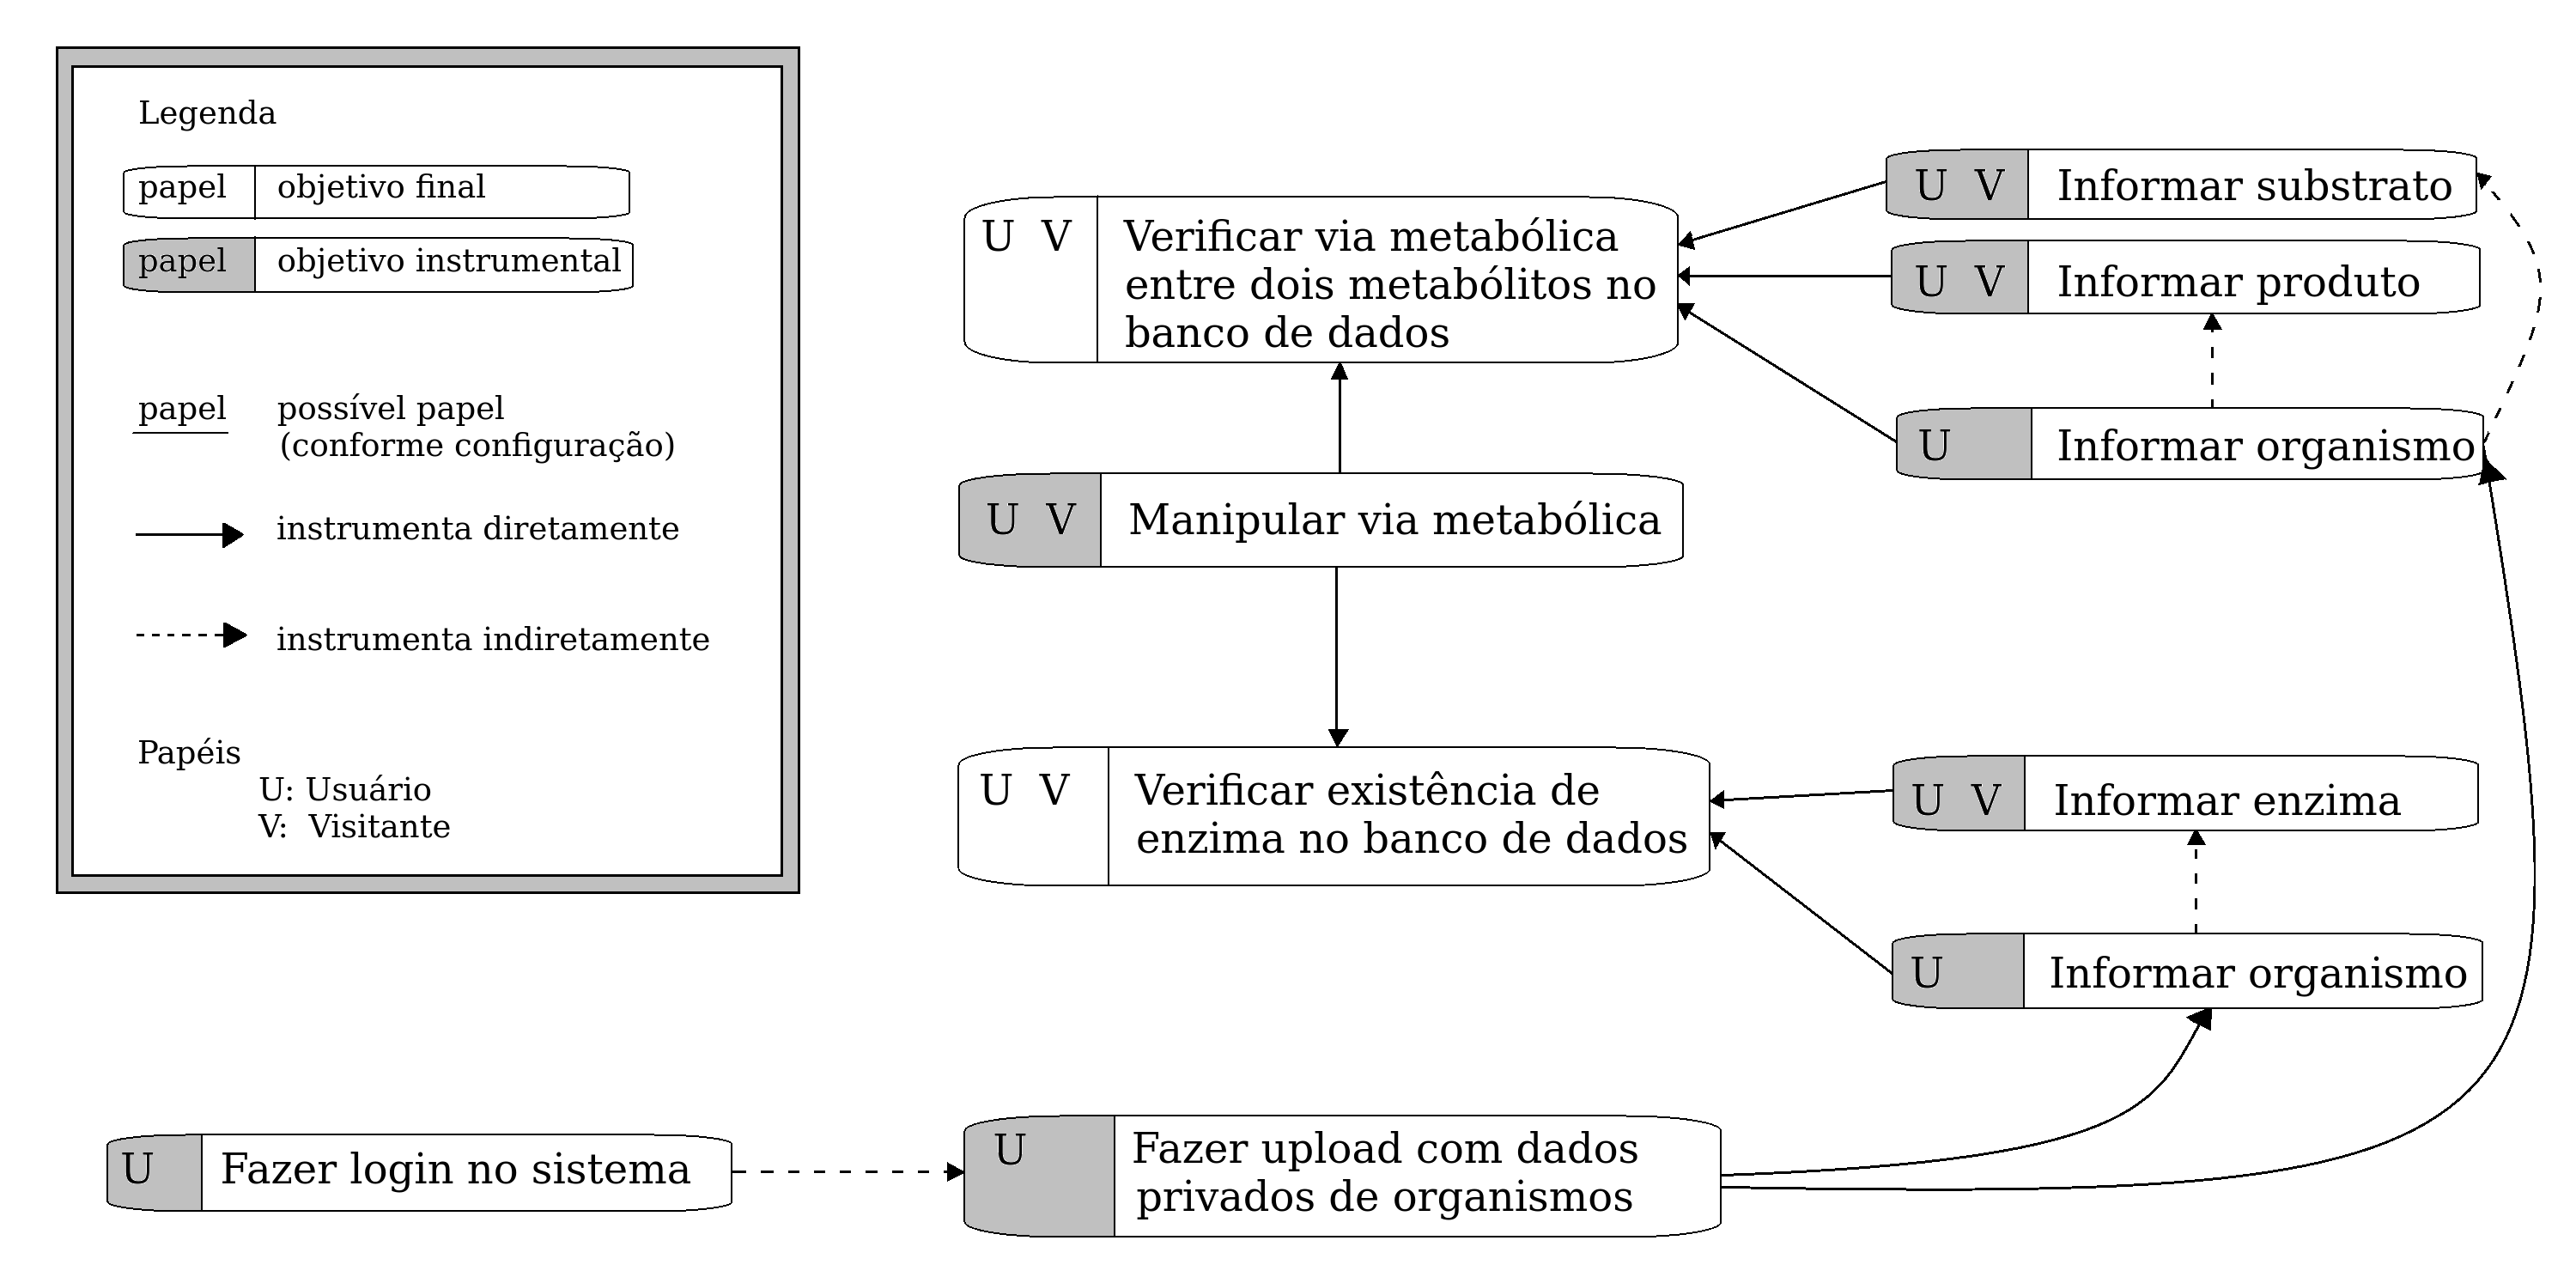
\includegraphics[width=1\textwidth]{mapaDeObjetivos.png}
    \caption{Mapa de Objetivos}
    \label{fig:mapaDeObjetivos}
\end{figure} 

\subsection{Modelagem de Tarefas}

\indent 

\begin{figure}[!h]
    \centering
    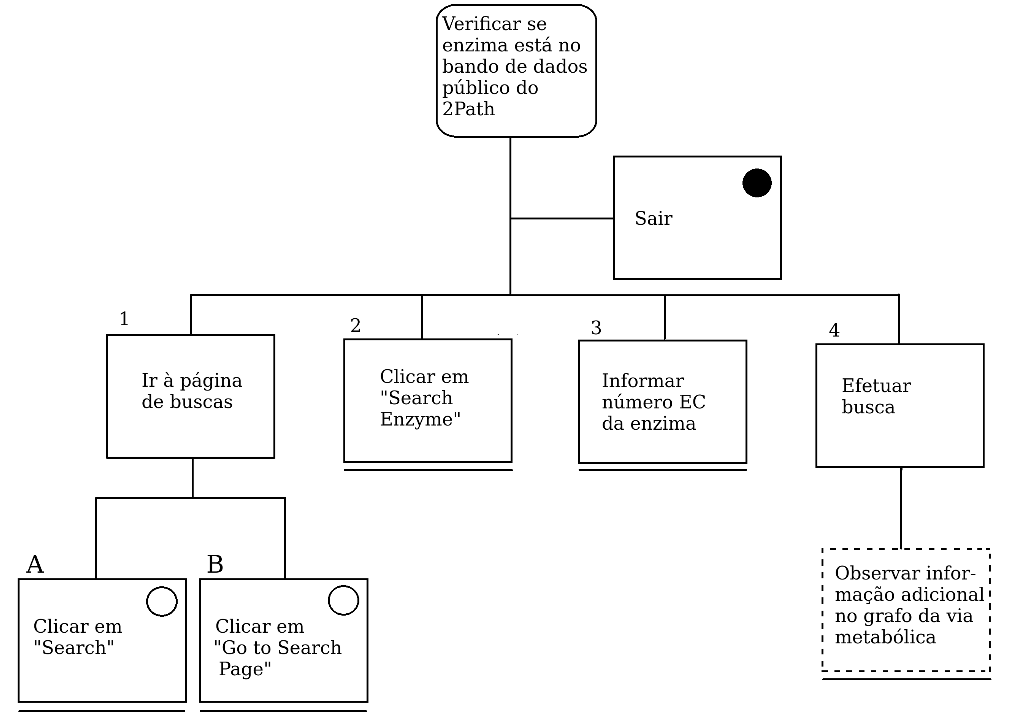
\includegraphics[width=0.8\textwidth]{objetivo_enzima.png}
    \caption{Objetivo de pesquisar enzima no banco de dados público.}
    \label{fig:objetivo_enzyma}
\end{figure}

\begin{figure}[!h]
    \centering
    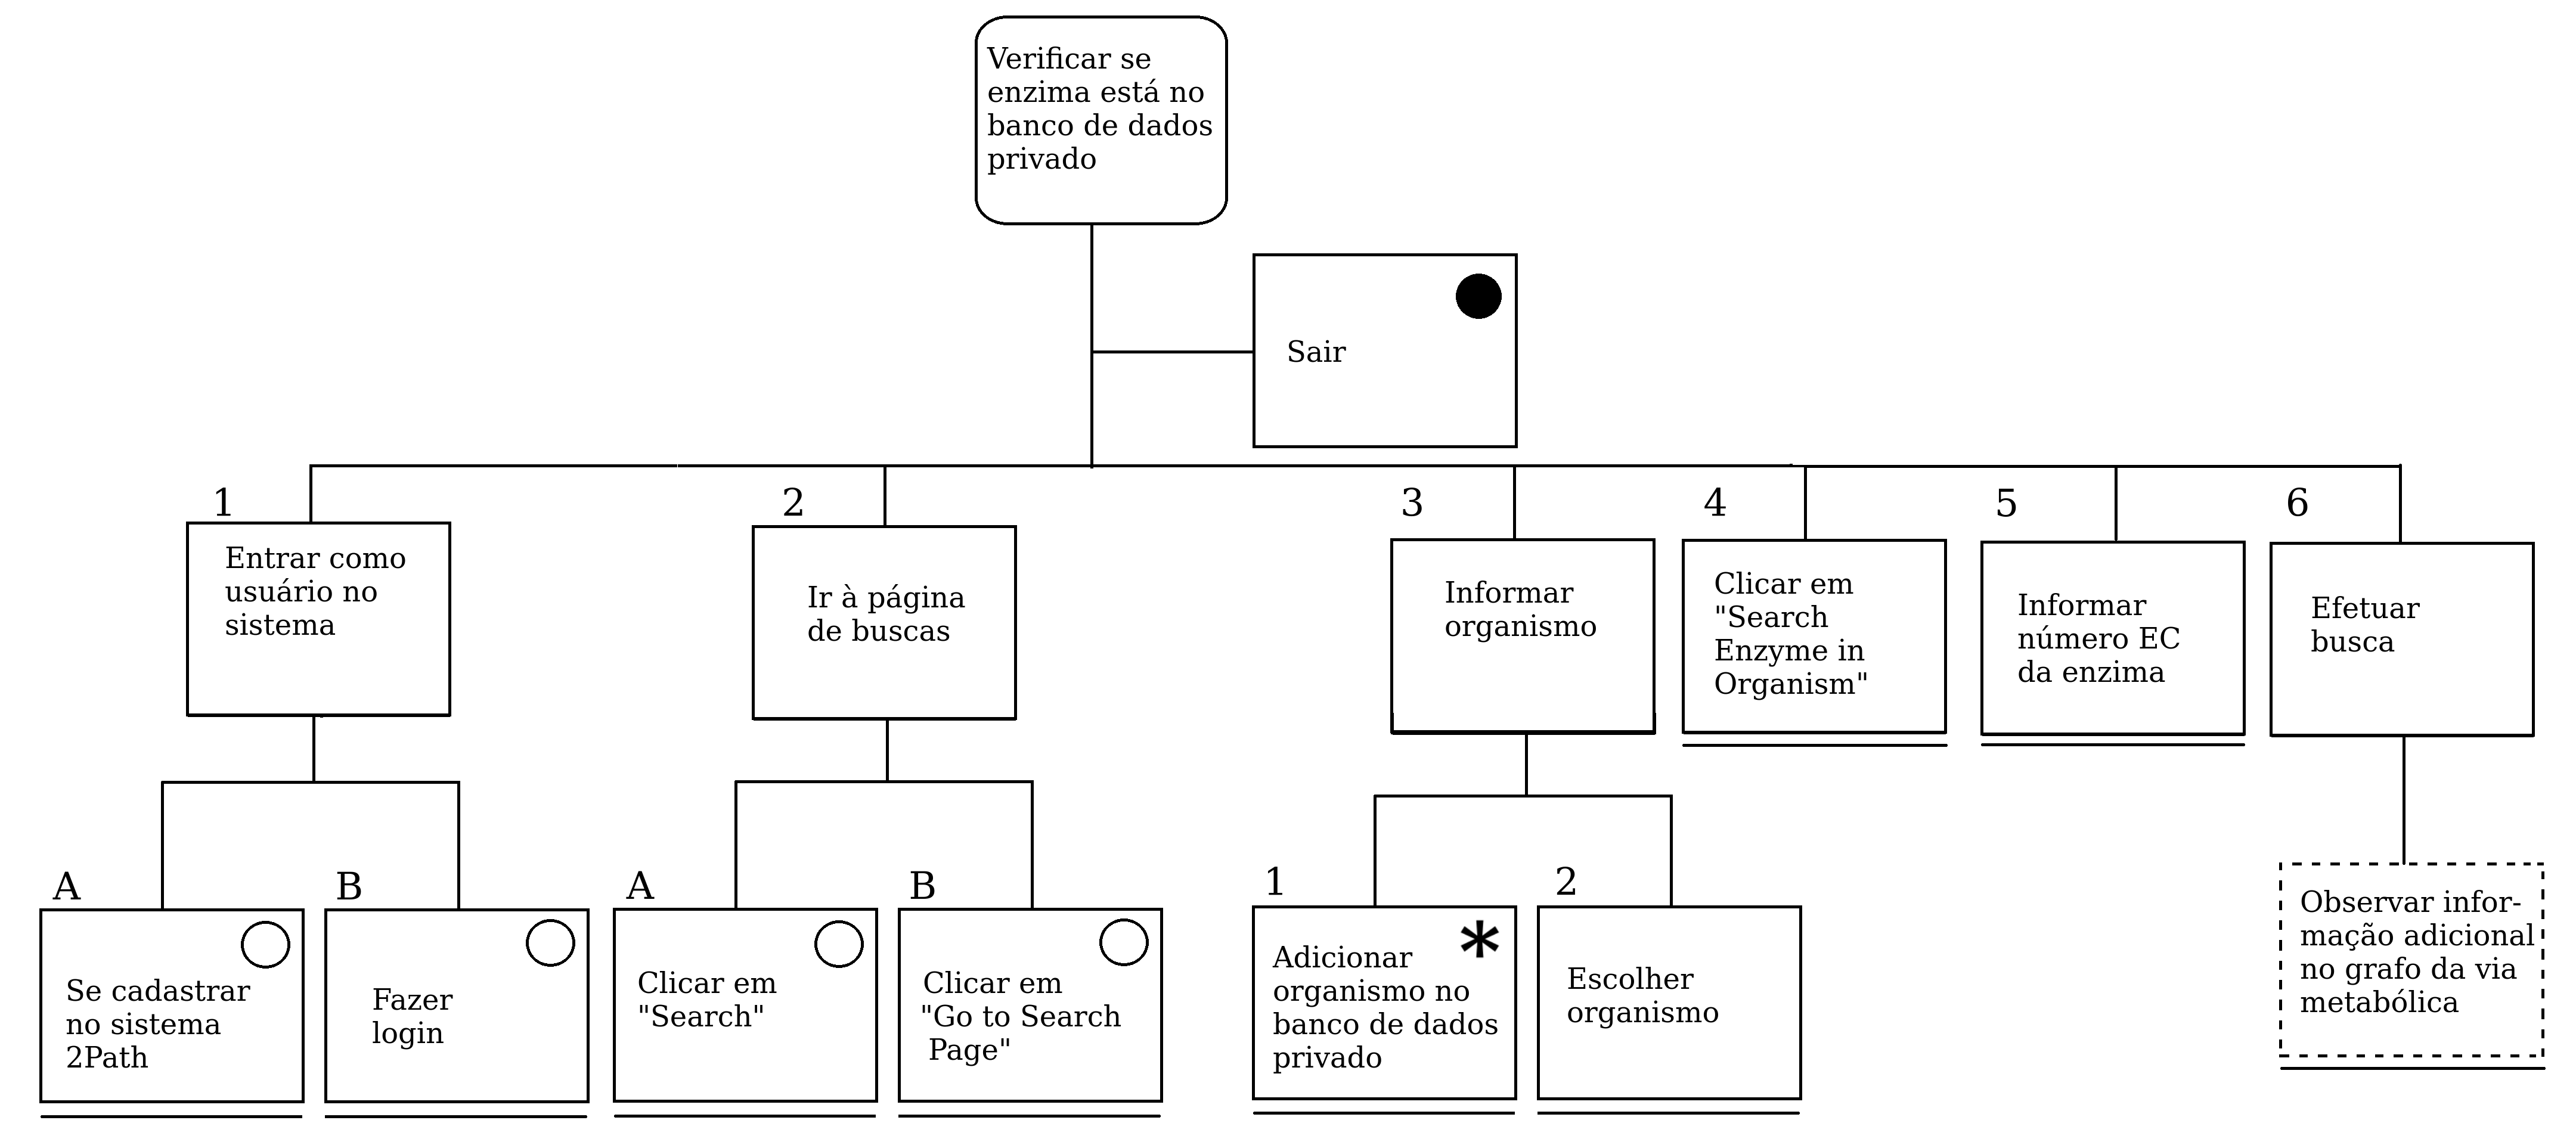
\includegraphics[width=1\textwidth]{objetivo_enzima_organismo.png}
    \caption{Objetivo de pesquisar enzima no banco de dados privado.}
    \label{fig:objetivo_enzyma_organismo}
\end{figure}

\begin{figure}[!h]
    \centering
    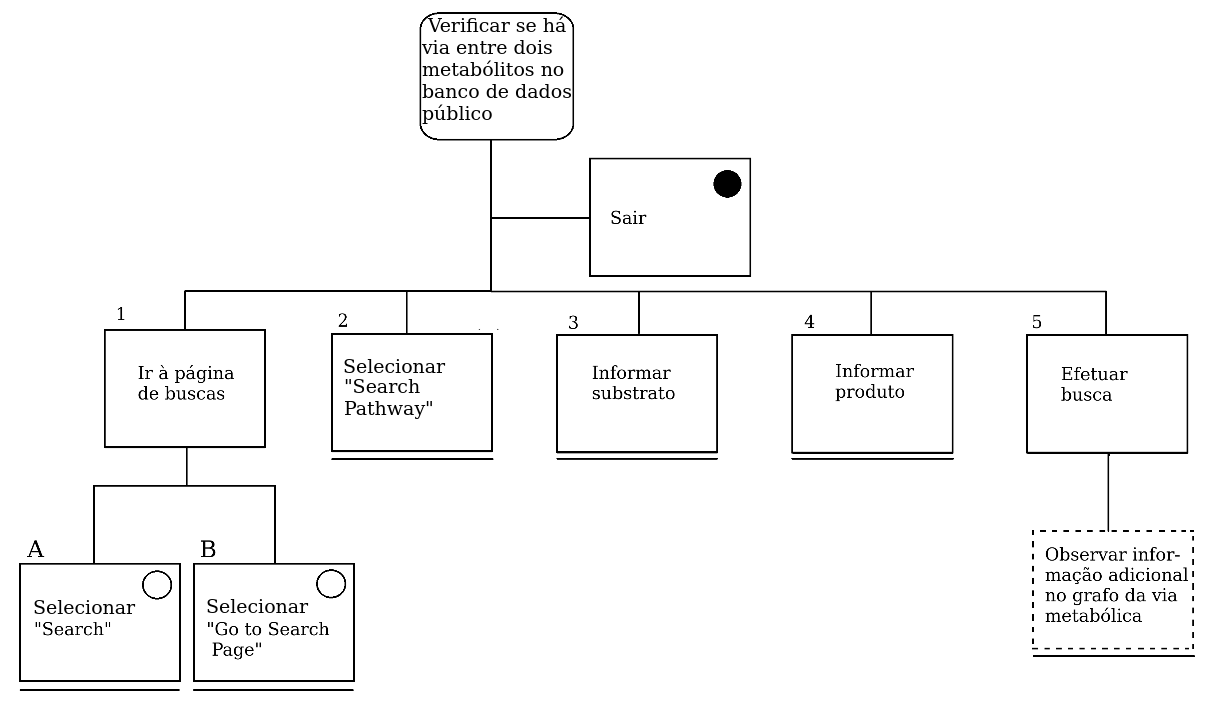
\includegraphics[width=1\textwidth]{objetivo_pathway.png}
    \caption{Objetivo de pesquisar via metabólica entre substrato e produto no banco de dados público.}
    \label{fig:objetivo_pathway}
\end{figure}

\begin{figure}[!h]
    \centering
    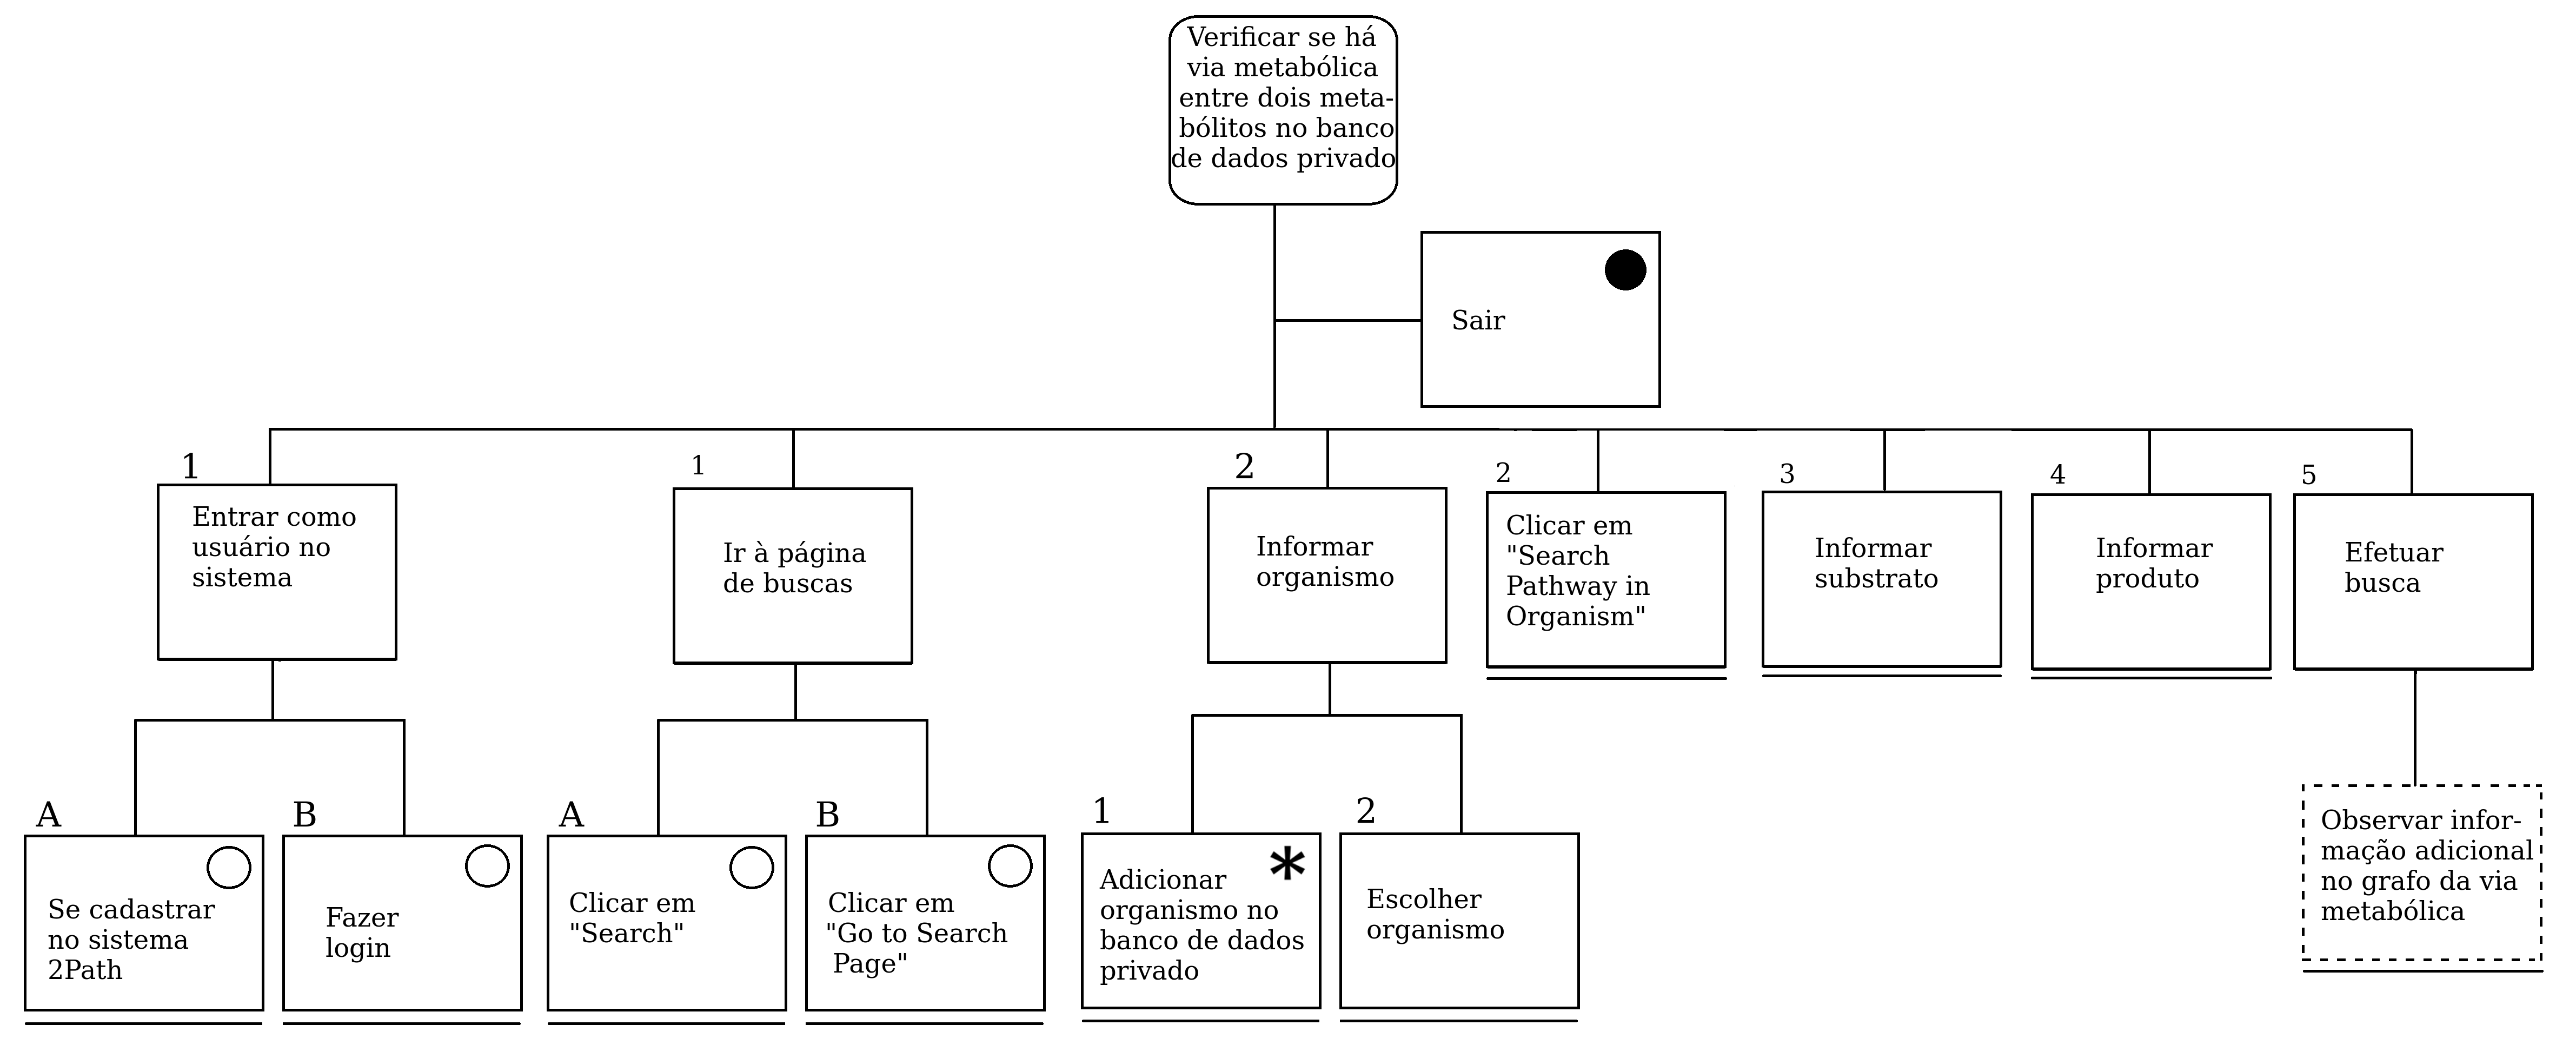
\includegraphics[width=1\textwidth]{objetivo_pathway_organismo.png}
    \caption{Objetivo de pesquisar via metabólica entre substrato e produto no banco de dados público.}
    \label{fig:objetivo_pathway_organismo}
\end{figure}

\subsection{Tratamento de Rupturas na Comunicação}

\indent 
\begin{table}
\centering
\caption{Campos de entrada e manipulação dos usuários do sistema 2Path} \label{prevencaoRecuperacao:2Path}
\begin{tabular}{|l|c|c|}
\hline
{\cellcolor[HTML]{DFDFDF}\textbf{Signo}} &  {\cellcolor[HTML]{DFDFDF}\textbf{Prevenção}} &  {\cellcolor[HTML]{DFDFDF}\textbf{Recuperação}}\\ \hline
\specialcell{Seleção de\\organismo}  & \specialcell{\textbf{PA}: Campo obrigatório com\\indicador ``*'' para\\ formulários ``\textit{Search Enzyme}\\\textit{in Organism}'' e  ``\textit{Search}\\\textit{Pathway in Organism}''. Caso\\o usuário esqueça de selecionar\\este campo, o organismo\\escolhido será o primeiro e\\ordem alfabética.} & -  \\ \hline

\specialcell{Seleção de\\enzima} & \specialcell{\textbf{PP}: Campo obrigatório com\\indicador ``*'';\\\textbf{PP}: Campo possui função\\\textit{auto-complete}, que fornece\\ao usuário todos os\\números EC existentes} & \specialcell{\textbf{RA}: Mensagem de texto em vermelho \\aparece acima do formulário informando\\o usuário de que o campo obrigatório\\não foi preenchido: ``\textit{Enzyme: Validation}\\\textit{ Error: Value is required}''.} \\ \hline

\specialcell{Seleção de\\substrato} & \specialcell{\textbf{PP}: Campo obrigatório com\\indicador ``*'';\\\textbf{PP}: Campo possui função\\\textit{auto-complete}, que fornece\\ao usuário todos os\\compostos existentes no\\2Path} & \specialcell{\textbf{RA}: Mensagem de texto em vermelho \\aparece acima do formulário informando\\o usuário de que o campo obrigatório\\não foi preenchido: ``\textit{From: Validation}\\\textit{Error: Value is required.}''.\\O ``From'' significa que a via\\tem início neste metabólito} \\ \hline

\specialcell{Seleção de\\produto} & \specialcell{\textbf{PP}: Campo obrigatório com\\indicador ``*'';\\\textbf{PP}: Campo possui função\\\textit{auto-complete}, que fornece\\ao usuário todos os\\compostos existentes no\\2Path} & \specialcell{\textbf{RA}: Mensagem de texto em vermelho \\aparece acima do formulário informando\\o usuário de que o campo obrigatório\\não foi preenchido: ``\textit{To: Validation}\\\textit{Error: Value is required.}''.\\O ``To'' significa que a via\\finaliza neste metabólito} \\ \hline

\specialcell{Manipulação\\da via\\metabólica} & - & - \\ \hline
\end{tabular}
\end{table}

% =========================================================================================

\section{Detalhes de Implementação}


\indent O sistema desenvolvido para este projeto é uma aplicação web chamada \textit{2Path}. O usuário deve se cadastrar no \textit{website} para ter acesso às redes metabólicas do banco de dados do sistema, bem como pesquisar por palavras chaves no mesmo. Nesta seção serão apresentadas as linguagens e ferramentas utilizadas no desenvolvimento do \textit{website}, as características, funcionalidades e limites do sistema e, por fim, as dificuldades enfrentadas na implementação do projeto.

\indent O sistema foi desenvolvido no amibiente de desenvolvimento integrado \textit{open source} Eclipse Java EE - \textit{Java Platform, Enterprise Edition}, versão Mars 4.5.2. Para simplificar a obtenção das dependências do projeto, ou seja, pacotes de arquivos java (extensão .jar), foi utilizada o Apache Maven\footnote{\textit{Software} de gerenciamento de projeto e ferramenta de compreensão de programa.}. Este \textit{software} opera sobre o arquivo \textit{pom.xml}, onde POM significa \textit{Project Object Model} e contém as especificações de cada projeto que se tornará dependência do sistema em desenvolvimento, além de outros aspectos do código. O servidor selecionado para hospedagem local, \textit{localhost} porta 8080, do sistema foi o Apache TomCat versão 7.0.

\indent As páginas da aplicação foram desenvolvidas na linguagem de marcação XHTML, \textit{Extensible Hypertext Markup Language}, e a estilzação em CSS, \textit{Cascading Style Sheets}. Para conexão entre \textit{front-end} e \textit{back-end} foram utilizados JSF\footnote{Especificação Java para criação de componentes de interface de aplicação \textit{web}.}, Primefaces\footnote{Biblioteca com uma coleção de componentes de interface voltadas para JSF.}, e AngularJS, para a construção do grafo de vias metabólicas.

\indent JSF: \url{https://projetos.inf.ufsc.br/arquivos_projetos/projeto_1214/Ferramenta\%20de\%20mapeamento\%20de\%20UIDs\%20para\%20JSF.pdf}

\indent CORES: \url{http://www.hermancerrato.com/graphic-design/images/color-images/the-meaning-of-colors-book.pdf}, \url{http://www.awwwards.com/trendy-web-color-palettes-and-material-design-color-schemes-tools.html}, \url{https://medium.com/wdstack/how-the-bootstrap-grid-really-works-471d7a089cfc#.k7w39z2uh}

% Communication websites which market to individual customers on a one-to-one basis would benefit with some blue in their marketing. Hi-tech and computer technology businesses can benefit from most shades of blue combined with gray.

\subsection{Banco de Dados Neo4j}


\subsection{Desafios}
 
O que foi o trabalho. 
Decrever todo o ambiente usado
Neste capítulo serão apresentados os primeiros resultados experimentais obtidos.

\section{Avaliação da Interface}

